\graphicspath{{chapters/images/01/}}


\chapter{Introduction}

\section{Transcriptomics}
\textbf{Transcriptome}: collection of mRNA species/transcripts in a cell at a given time\\

\subsection{Microarrays}
\textbf{Microarrays} can be used to measure levels of mRNA in a high-throughput fashion. Results of microarrays have to be normalized \cite{smythNormalizationCDNAMicroarray2003}
\\
Transcriptomics is \textbf{robust}, relatively \textbf{cost effective} and \textbf{user friendly}
\\
Genes with different expressions can be visualized, each column is a sample and each row is one of the 25 genes. The colour represents the level of expression. How much difference there has to be?


\begin{figure}[h]
\caption{}
\centering
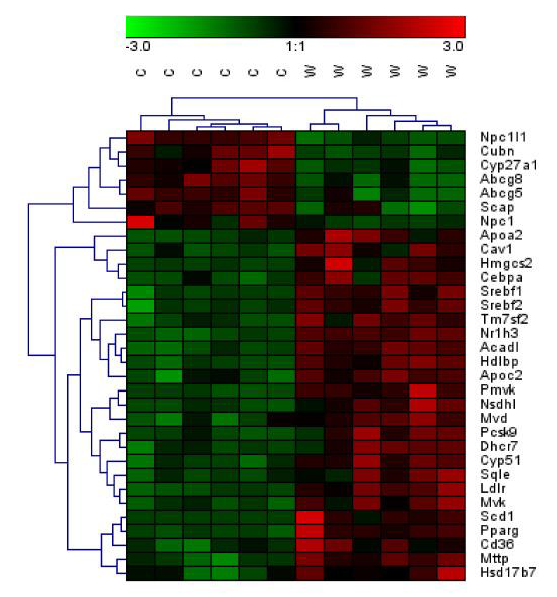
\includegraphics[width=0.6\textwidth]{MicroRNAresults}
\end{figure}

\subsection{Next generation sequencing}
Similar in concept to microarrays, but instead of hybridizing sample to a set
of probes, each mRNA species in each sample is broken into fragments, and
all fragments are sequenced base by base. The current technologies manage to sequence small pieces of RNA, around 250 bases. By using the ends of the fragments, they can be obtained whole areas that can permit to reassamble RNAs. A lot of fragments are prefearable for an higher coverage.


\subsection{RNA-seq pipeline}
3 input files are requested: input raw data file, a reference genome and some gene annotations. Some cloud services can be used

\begin{figure}[h]
\caption{}
\centering
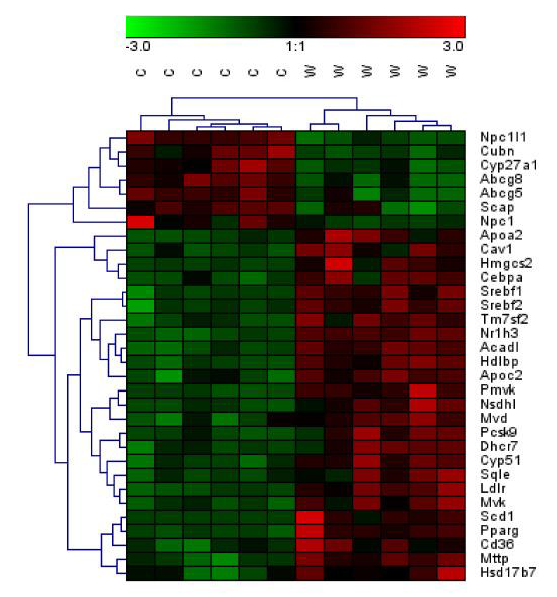
\includegraphics[width=0.6\textwidth]{MicroRNAresults}
\end{figure}

\subsection{Microarrays vs Sequencing}

\begin{figure}[h]
\caption{}
\centering
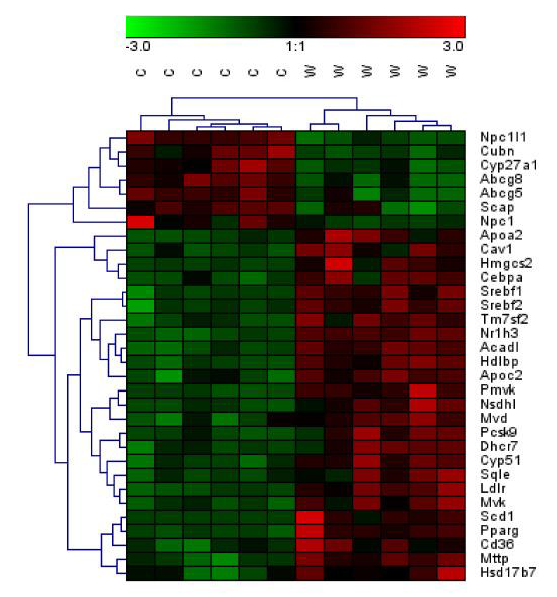
\includegraphics[width=0.6\textwidth]{MicroRNAresults}
\end{figure}


\section{Proteomics}
Quantification of proteins level, 3 main technologies:
\begin{itemize}
\item 2D gel electrophoresys
\item liquid chromatography mass spectrometry
\item protein array
\end{itemize}

2D gel electrophoresys is one of the most common techniques, proteins are divided through weight, different charges. Through the isoelectric method, proteins migrate towards their isoelectric pH. In this way.


\begin{figure}[h]
\caption{}
\centering
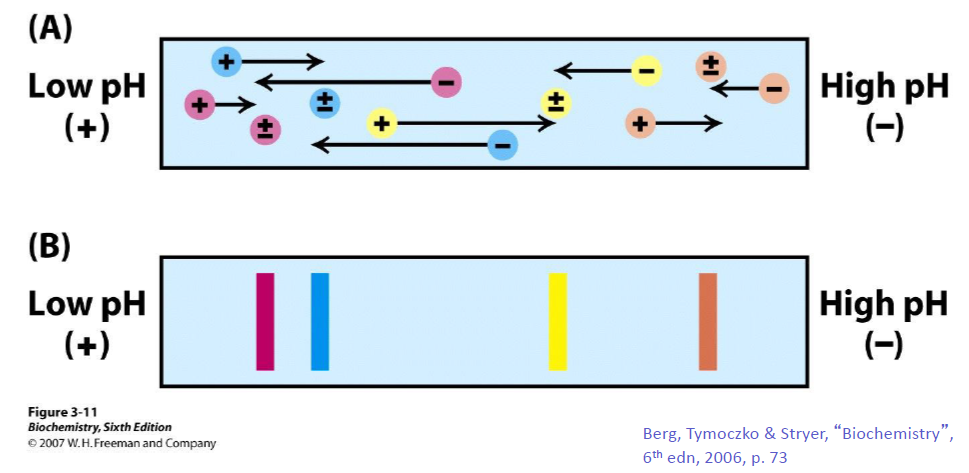
\includegraphics[width=0.6\textwidth]{IsoelectricProteinSeparation}
\end{figure}

Mass spectrometry measures the ration between mass and electrical charge. It is shown the relative abundance of the fragments. Chromatography can be done at first, another tecnique which ... . Then it has to be rebuilt the original composition of the protein. Very laborious\\

\textbf{Protein arrays} are made through aptameters, which are oligonucleotides or peptide molecules designed to uniquely bind to a specific molecule. The protein binds to the aptamer and a fluorescenct signal is produced .
This technology is easy and cheap, but measures a low amount of proteins, and of those an aptamer was found. It is today an emergent technology \cite{neaguProteinMicroarrayTechnology2019}.

\begin{figure}[h]
\caption{}
\centering
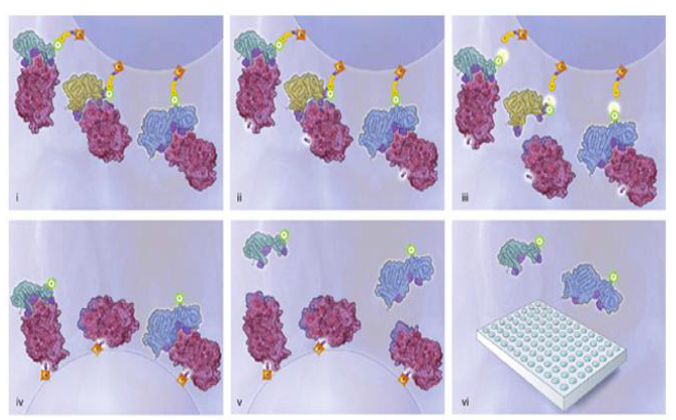
\includegraphics[width=0.6\textwidth]{ProteinArray}
\end{figure}

Proteomics still relatively \textbf{limited} problems can remain with purification and
stability of proteins

\section{Metabolomics}
\textbf{Metabolomics}: A field of life science research that uses High Throughput
(HT) technologies to identify and/or characterize all the small molecules or
metabolites in a given cell, tissue or organism (i.e. the metabolome
\\
Metabolomics can be done in two ways: Through a quantitative methos, or chemometric method 

%approfondire metabolomica
%TODO

\section{Microbiome}
%TODO

\section{Other high-throughput data}
\subsection{Epigenomics}
\textbf{Epigenetics} is the study of heritable changes in gene
activity that are not caused by changes in the DNA sequence. Some mechanisms that produce such changes are
\textit{DNA methylation} and \textit{histone modification}. Both mechanisms alters how genes are expressed without
altering the underlying DNA sequence.

\begin{figure}[h]
\caption{}
\centering
\includegraphics[width=0.6\textwidth]{EuEtChromatin}
\end{figure}

\subsection{Micro RNA}
affects translation of mRNA, the miRNA of humans are around 1000, they are formed by 20-22 bases. After being synthesized inside the nucleus as a precursor, a miRNA molecule is modified ... %TODO
\\
MicroRNA profiles are really common, it is possible to do an additional step: some specific programs relate miRNA molecules to genes that are being regulated.

\subsection{Protein Protein interaction - Interactome}
Databases of interactions are available\\

Interactomes are shown normally in 3D graphs, with nodes representing proteins, and the lines the interactions between each of them.	


\section{Clinical Trial study design}
with a cell line or a model organism. Hundreds of cell-lines, and some of them  are immortalized.


%I wrote the things the professor talked about. Some things are basic for me and I neglect them. Some slides are missing %TODO
